\documentclass[hyperref={hidelinks}]{beamer}
\usetheme[sectionpage=none,numbering=fraction,progressbar=frametitle]{metropolis}
\usepackage{booktabs}
\usepackage{multirow}
\graphicspath{{figures/}}

\title{Aprendizagem Aplicada à Segurança}
\date{\today}

\author{Mário Antunes}
\institute{University of Aveiro}

\begin{document}
  \maketitle

  \begin{frame}{Table of Contents}
    \tableofcontents
  \end{frame}

  \section{SPAM}
  \begin{frame}{SPAM}
    \begin{itemize}
      \item The term ``spam'' is internet slang that refers to unsolicited commercial email (UCE).
      \item The first reported case of spam occurred in 1898, when the New York Times reported unsolicited messages circulating in association with an old swindle.
      \item The term ``spam'' was coined in 1994, based on a now-legendary Monty Python's Flying Circus sketch, where a crowd of Vikings sings progressively louder choruses of ``SPAM! SPAM! SPAM!''
    \end{itemize}
  \end{frame}

  \begin{frame}{SPAM}
    \begin{figure}
    \centering
    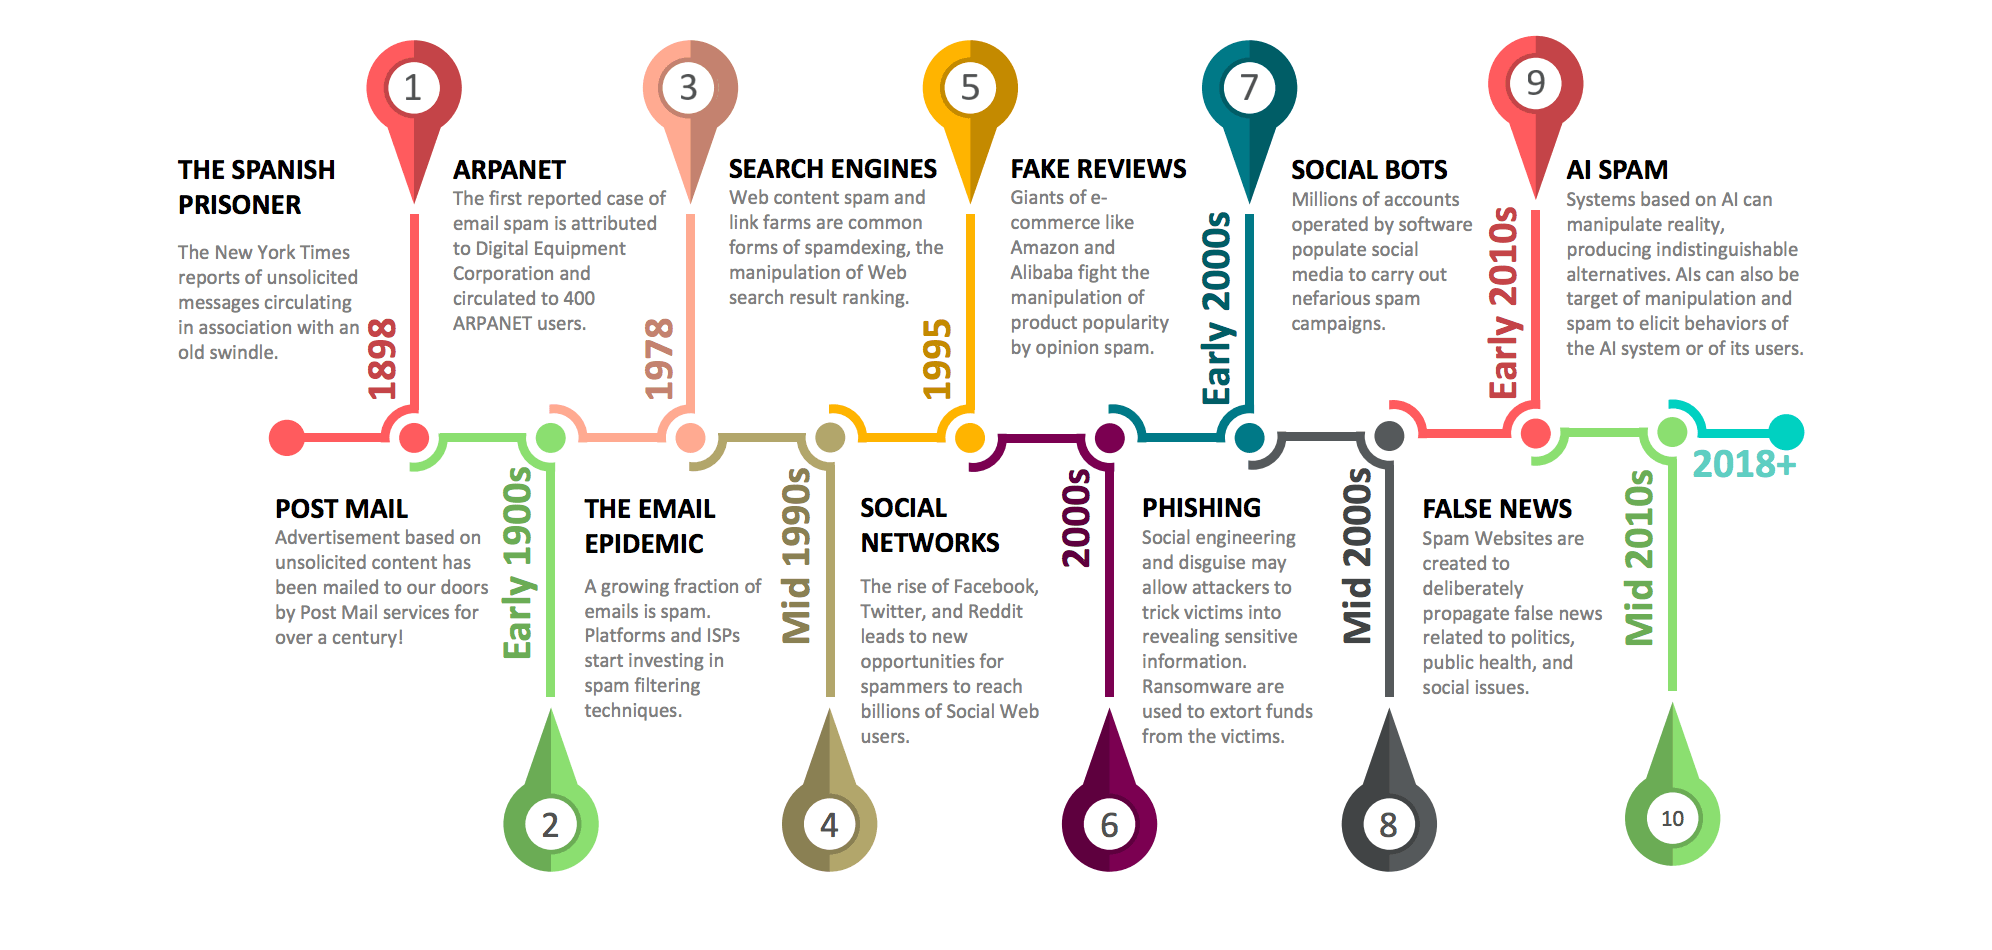
\includegraphics[width=\textwidth]{spam_history}
    \end{figure}
  \end{frame}

  \begin{frame}{SPAM}
    \begin{figure}
    \centering
    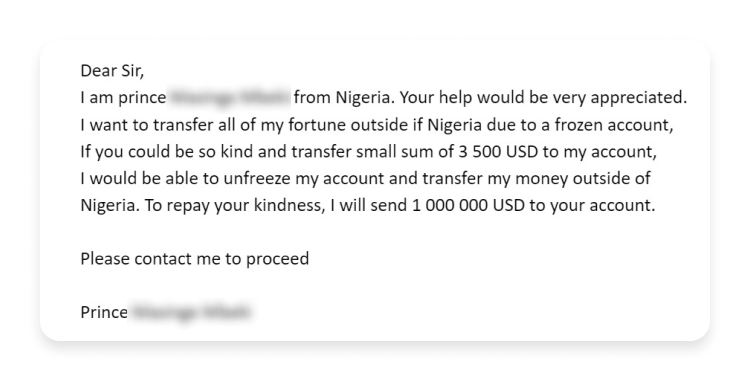
\includegraphics[width=.8\textwidth]{nigerian-prince-scam}
    \end{figure}
  \end{frame}
  
  \begin{frame}{Fight against SPAM}
    \begin{itemize}
      \item \emph{Huge} list of \href{anti-spam techniques}{\url{https://en.wikipedia.org/wiki/Anti-spam_techniques}}
      \item From common sense to \emph{Bayesian spam filtering}
      \item Unfortunately it is a costly battle
    \end{itemize}
  \end{frame}

  \begin{frame}{Fight against SPAM}
    \begin{figure}
    \centering
    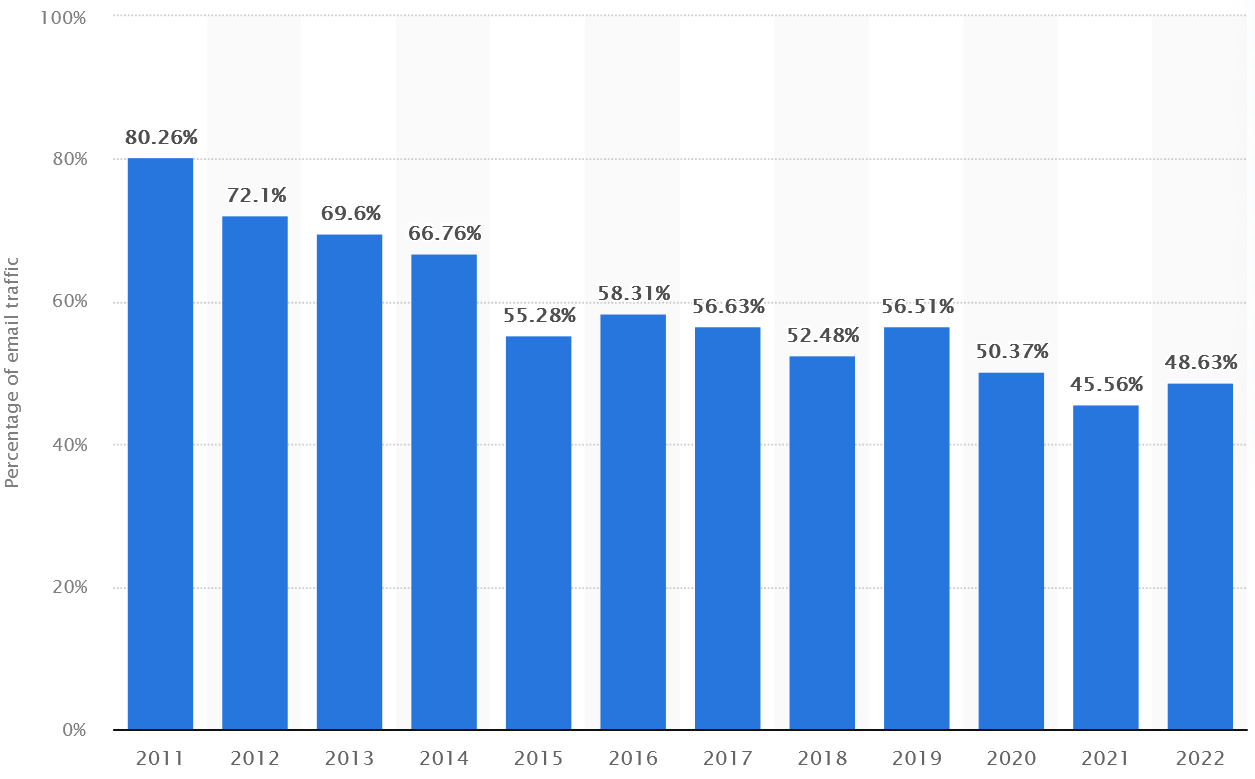
\includegraphics[width=.8\textwidth]{spam-traffic}
    \end{figure}
  \end{frame}

  \section{SPAM Detection}
  \begin{frame}{SPAM Detection}
    \begin{figure}
    \centering
    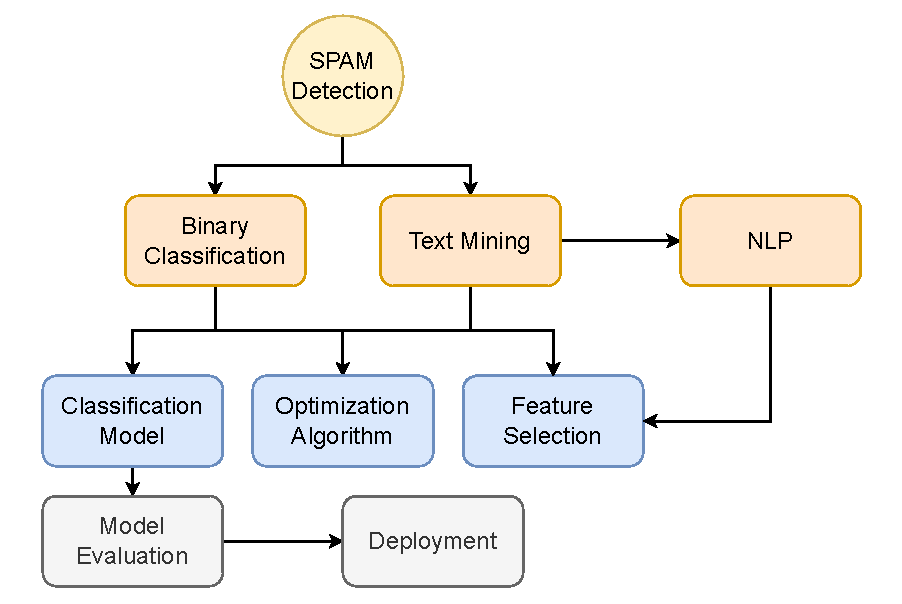
\includegraphics[width=\textwidth]{spam.drawio}
    \end{figure}
  \end{frame}

  \section{Binary Classification}
  \begin{frame}{Binary Classification}
    \begin{itemize}
      \item Binary classification is the task of classifying the elements of a set into two groups (each called class) on the basis of a classification rule.
      \item For this application one message can either be spam or ham.
    \end{itemize}
    \begin{figure}
    \centering
    
\includegraphics[width=.6\textwidth]{Binary-Classification}
    \end{figure}
  \end{frame}

  \section{Text Mining}
  \begin{frame}{Text Mining}
    \begin{itemize}
      \item Text mining is the process of deriving high-quality information from text.
      \item Combines concepts from Machine Learning, Linguistic and statistical analysis.
      \item In this area we will explore the methods used to rank words\slash tokens and the BoW model.
    \end{itemize}
  \end{frame}

  \begin{frame}{Bag of Words (Bow) model}
    \begin{figure}
    \centering
    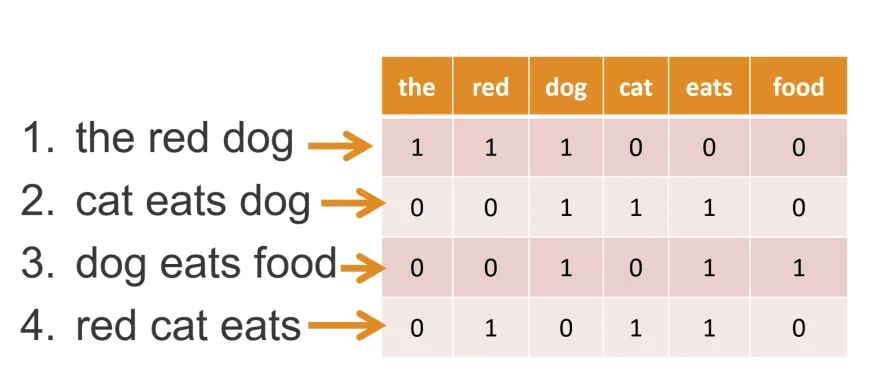
\includegraphics[width=.6\textwidth]{bow}
    \end{figure}
  \end{frame}

  \section{Natural Language Processing (NLP)}
  \begin{frame}{Natural Language Processing (NLP)}
    \begin{itemize}
      \item NLP gives the computers the ability to understand text.
      \item Combines \emph{Sintax} and \emph{Semantic} into the analysis.
      \item One famous exemples are the Large Language Models (LLMs) that power OpenAI Chat GPT.
    \end{itemize}
  \end{frame}

  \section{Classification Model}
  \begin{frame}{Classification Model}
    \begin{itemize}
      \item SPAM detection is ``considered'' a toy example.
      \item As such, we will explore two of the simples learning models: Naive Bayes and Logistic Regression.
    \end{itemize}
    \begin{columns}
      \column{0.5\textwidth}
      \begin{figure}
        \centering
        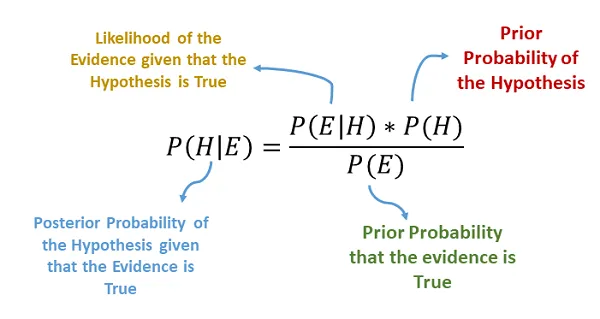
\includegraphics[width=\textwidth]{NB}
        \end{figure}
      \column{0.5\textwidth}
      \begin{figure}
        \centering
        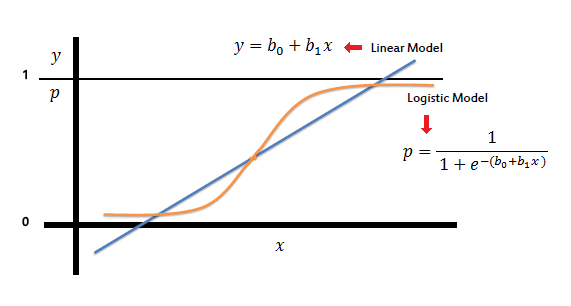
\includegraphics[width=\textwidth]{LogReg}
        \end{figure}
    \end{columns}
  \end{frame}

  \section{Model Evaluation}
  \begin{frame}{Model Evaluation}
    \begin{itemize}
      \item Classification model can be evaluated using a confusing matrix
      \item The simplest methods to evaluate a model is throuhgh accuracy: $acc = \frac{TP+TN}{TN+TN+FP+FN}$
    \end{itemize}
    \begin{figure}
    \centering
    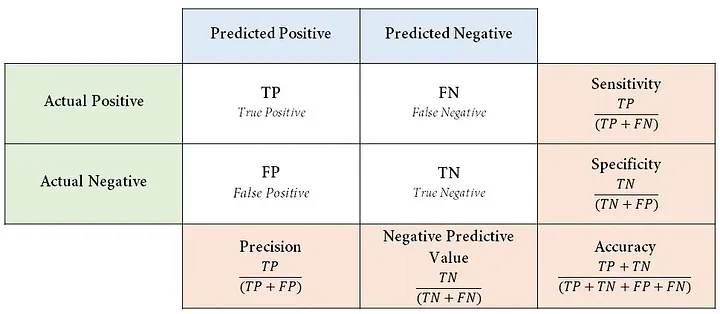
\includegraphics[width=.7\textwidth]{CM}
    \end{figure}
  \end{frame}

  \begin{frame}{Model Evaluation}
    \begin{figure}
    \centering
    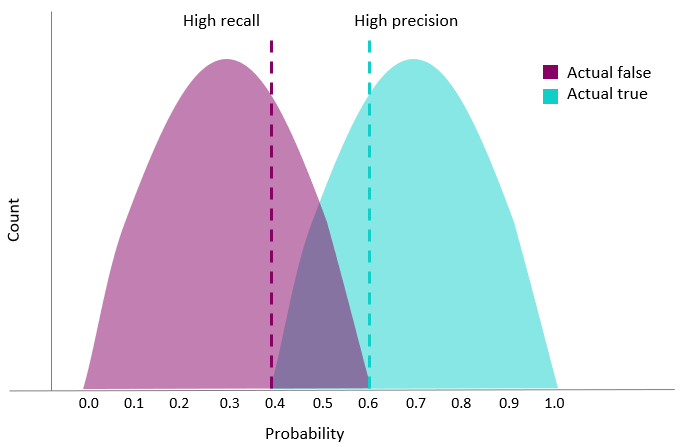
\includegraphics[width=.7\textwidth]{acc}
    \end{figure}
  \end{frame}

\end{document}